%http://www.itdaan.com/blog/2013/11/07/1dd004fe08f7989a48b40caed6fa057c.html
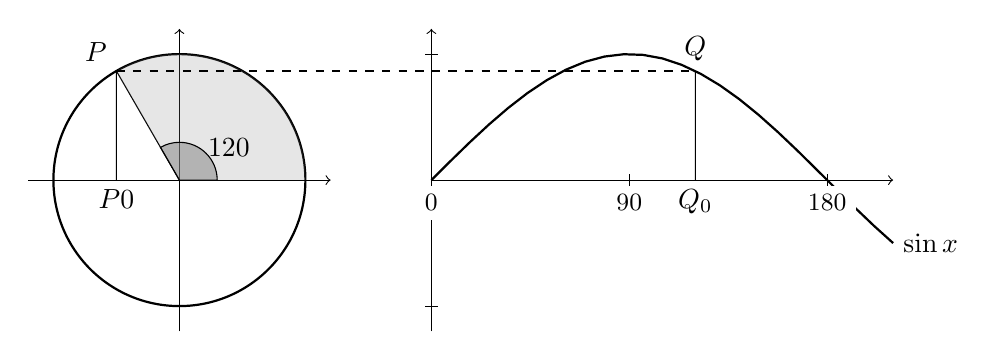
\begin{tikzpicture}[scale=1.6]
\def\iangle{120}
\begin{scope}[xshift=-2cm]
\draw[->] (-1.2,0) --(1.2,0);
\draw[->] (0,-1.2) --(0,1.2);
\draw[thick] (0,0) circle(1cm);
\coordinate [label = \iangle:$P$] (P) at (\iangle:1);
\coordinate [label = below:$P0$] (P0) at (P |-0,0);
\draw (P)--(P0);
\draw (0,0)--(P);
\fill [fill = gray,fill opacity=0.2] (0,0)--(0:1) arc (0:\iangle:1)--cycle;
\filldraw [fill = gray,fill opacity=0.5] (0,0)--(0:0.3) arc (0:\iangle:0.3)--cycle;
\node [right] at (\iangle/2:0.3) {\ang{\iangle}};

\end{scope}

\draw[->] (0,0) --({rad(210)},0);
\draw[->] (0,-1.2) --(0,1.2);
\draw [thick,domain=0:rad(210)] plot (\x,{sin(\x r)}) node [right] {$\sin x$};

\foreach \t in {0,90,180}
{
\draw ({rad(\t)},-0.05)--({rad(\t)},0.05) ;
\node [below,outer sep =2pt ,font=\small , fill = white] at ({rad(\t)},0) {\ang{\t}};
}
\foreach \y in {-1,1}
{
\draw (-0.05,\y) -- (0.05,\y);
}

\coordinate [label=above:{$Q$}] (Q) at ({rad(\iangle)},{sin(\iangle)});
\coordinate [label=below:{$Q_0$}] (Q0) at (Q |- 0,0);
\draw (Q)--(Q0);
\draw[dashed] (P) --(Q);




\end{tikzpicture}